\chapter{Unsupervised Learning}

\begin{definitionblock}[Unsupervised Learning]
Unsupervised Learning is a type of machine learning that looks for previously undetected patterns in a data set with no pre-existing labels and with a minimum of human supervision.
\end{definitionblock}

\section{Clustering}

We assume that the system that generated the data followed some scheme (\textbf{pattern}), we do not know it and we want to discover it from a dataset.

\begin{itemize}
    \item the example is the dataset $P^{*}(X)$
    \item what we learn from the dataset is not, in general, usable in another dataset $\to$ \textbf{find} patterns is fairer than \textbf{learn} patterns
\end{itemize}

We first look for a \textbf{grouped} data, but we do not know the groups. This is the \textbf{clustering} problem.

\begin{definitionblock}[Clustering]
Clustering is the task of grouping a set of objects in such a way that objects in the same group (called a cluster) are more similar to each other than to those in other groups.
\end{definitionblock}

Given a dataset $D \in P^*(X)$, find a partitioning $\{D_1,\dots,D_k\}$ such that each $D_i$ is a cluster.

\begin{itemize}
    \item close toghether?
    \item how close?
    \item where does k come from?
\end{itemize}

This is an optimization problem, where for any k,d, there exists at least one optimal solution. In principle one can try all the partitions and measure the distance, but in practice k is unknown and trying all the partitions is unfeasible.

\begin{center}
    $\operatorname*{argmax}_{D_1,\dots,D_k}(\sum \sum d(x,x'))-(\sum\sum d(x,x'))$

    subject to $\bigcup D_i = D$ and $D_i \cap D_j = \emptyset$
\end{center}

\begin{itemize}
    \item \textbf{maximize} the distance between any two $x,x'$ when they belong to different clusters
    \item minimize the distance between any two $x,x'$ when they belong to the same cluster
    \item clusters ave to form a partition
\end{itemize}

Can't be also optimized k? No, it is pointless.
\begin{itemize}
    \item $k = 1 \to $no clustering
    \item $k = n \to $each point is a cluster
\end{itemize}

\begin{figure}[H]
    \centering
    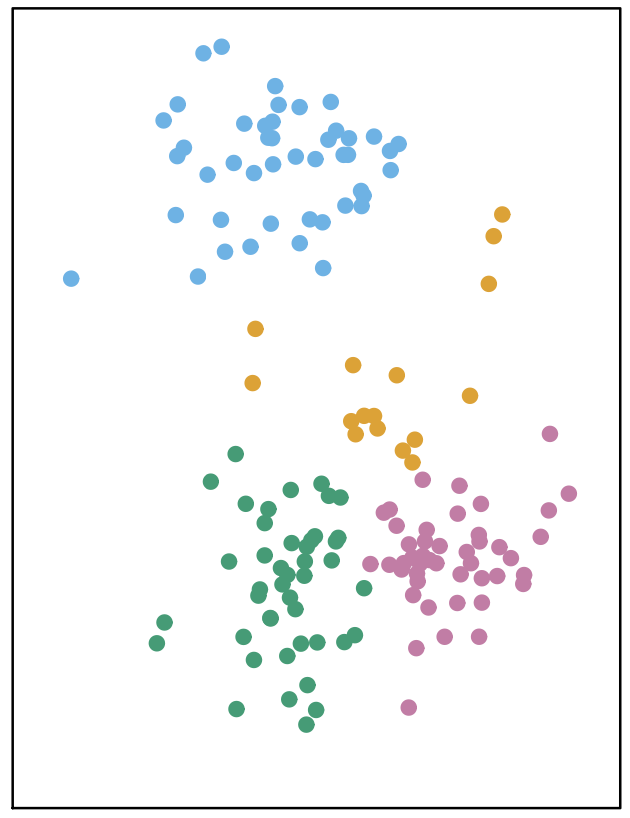
\includegraphics[width=0.5\textwidth]{assets/fig35.png}
    \caption{Clustering}
\end{figure}

How to access clustering in practice?
\begin{itemize}
    \item inspect D manually
    \item insert the clustering inside the larger information processyng system and measure some other indexes
    \item measure some performance indexes 
\end{itemize}

\begin{exampleblock}[Performance Index: Silhouette Index]
It considers, form each observation, the average distance to the observations in the same cluster and the min distance to the observations in other clusters.
\begin{itemize}
    \item $a(i) = \frac{1}{|D_i|} \sum_{x \in D_i} d(x,D_i)$
    \item $b(i) = \min_{j \neq i} \frac{1}{|D_j|} \sum_{x \in D_j} d(x,D_i)$
    \item $s(i) = \frac{b(i)-a(i)}{\max(a(i),b(i))}$
    \item $S = \frac{1}{n} \sum s(i)$
\end{itemize}
The index is between -1 and 1, where 1 is the best clustering. The larger the index, the better the clustering.
\end{exampleblock}

\newpage
\subsection{Hierarchical Clustering}

\begin{definitionblock}[Hierarchical Clustering]
It is an iterative method in which:
\begin{itemize}
    \item at each j-th iteration, there exist a partition $D_1,\dots,D_{k_j}$
    \item at most two clusters differ between partitions at subsequent iterations
    \item you do not set k 
\end{itemize}
It is of two types:
\begin{itemize}
    \item \textbf{Agglomerative}: start with each point as a cluster and merge the closest clusters
    \item \textbf{Divisive}: start with all the points in a cluster and split the farthest points
\end{itemize}
\end{definitionblock}

Cluster distance can be computed in different ways:
\begin{itemize}
    \item \textbf{Single Linkage}: the distance between two clusters is the distance between the closest points in the two clusters
    \item \textbf{Complete Linkage}: the distance between two clusters is the distance between the farthest points in the two clusters
    \item \textbf{Average Linkage}: the distance between two clusters is the average distance between all the points in the two clusters
    \item \textbf{Centroid Linkage}: the distance between two clusters is the distance between the centroids of the two clusters
\end{itemize}

\begin{figure}[H]
    \centering
    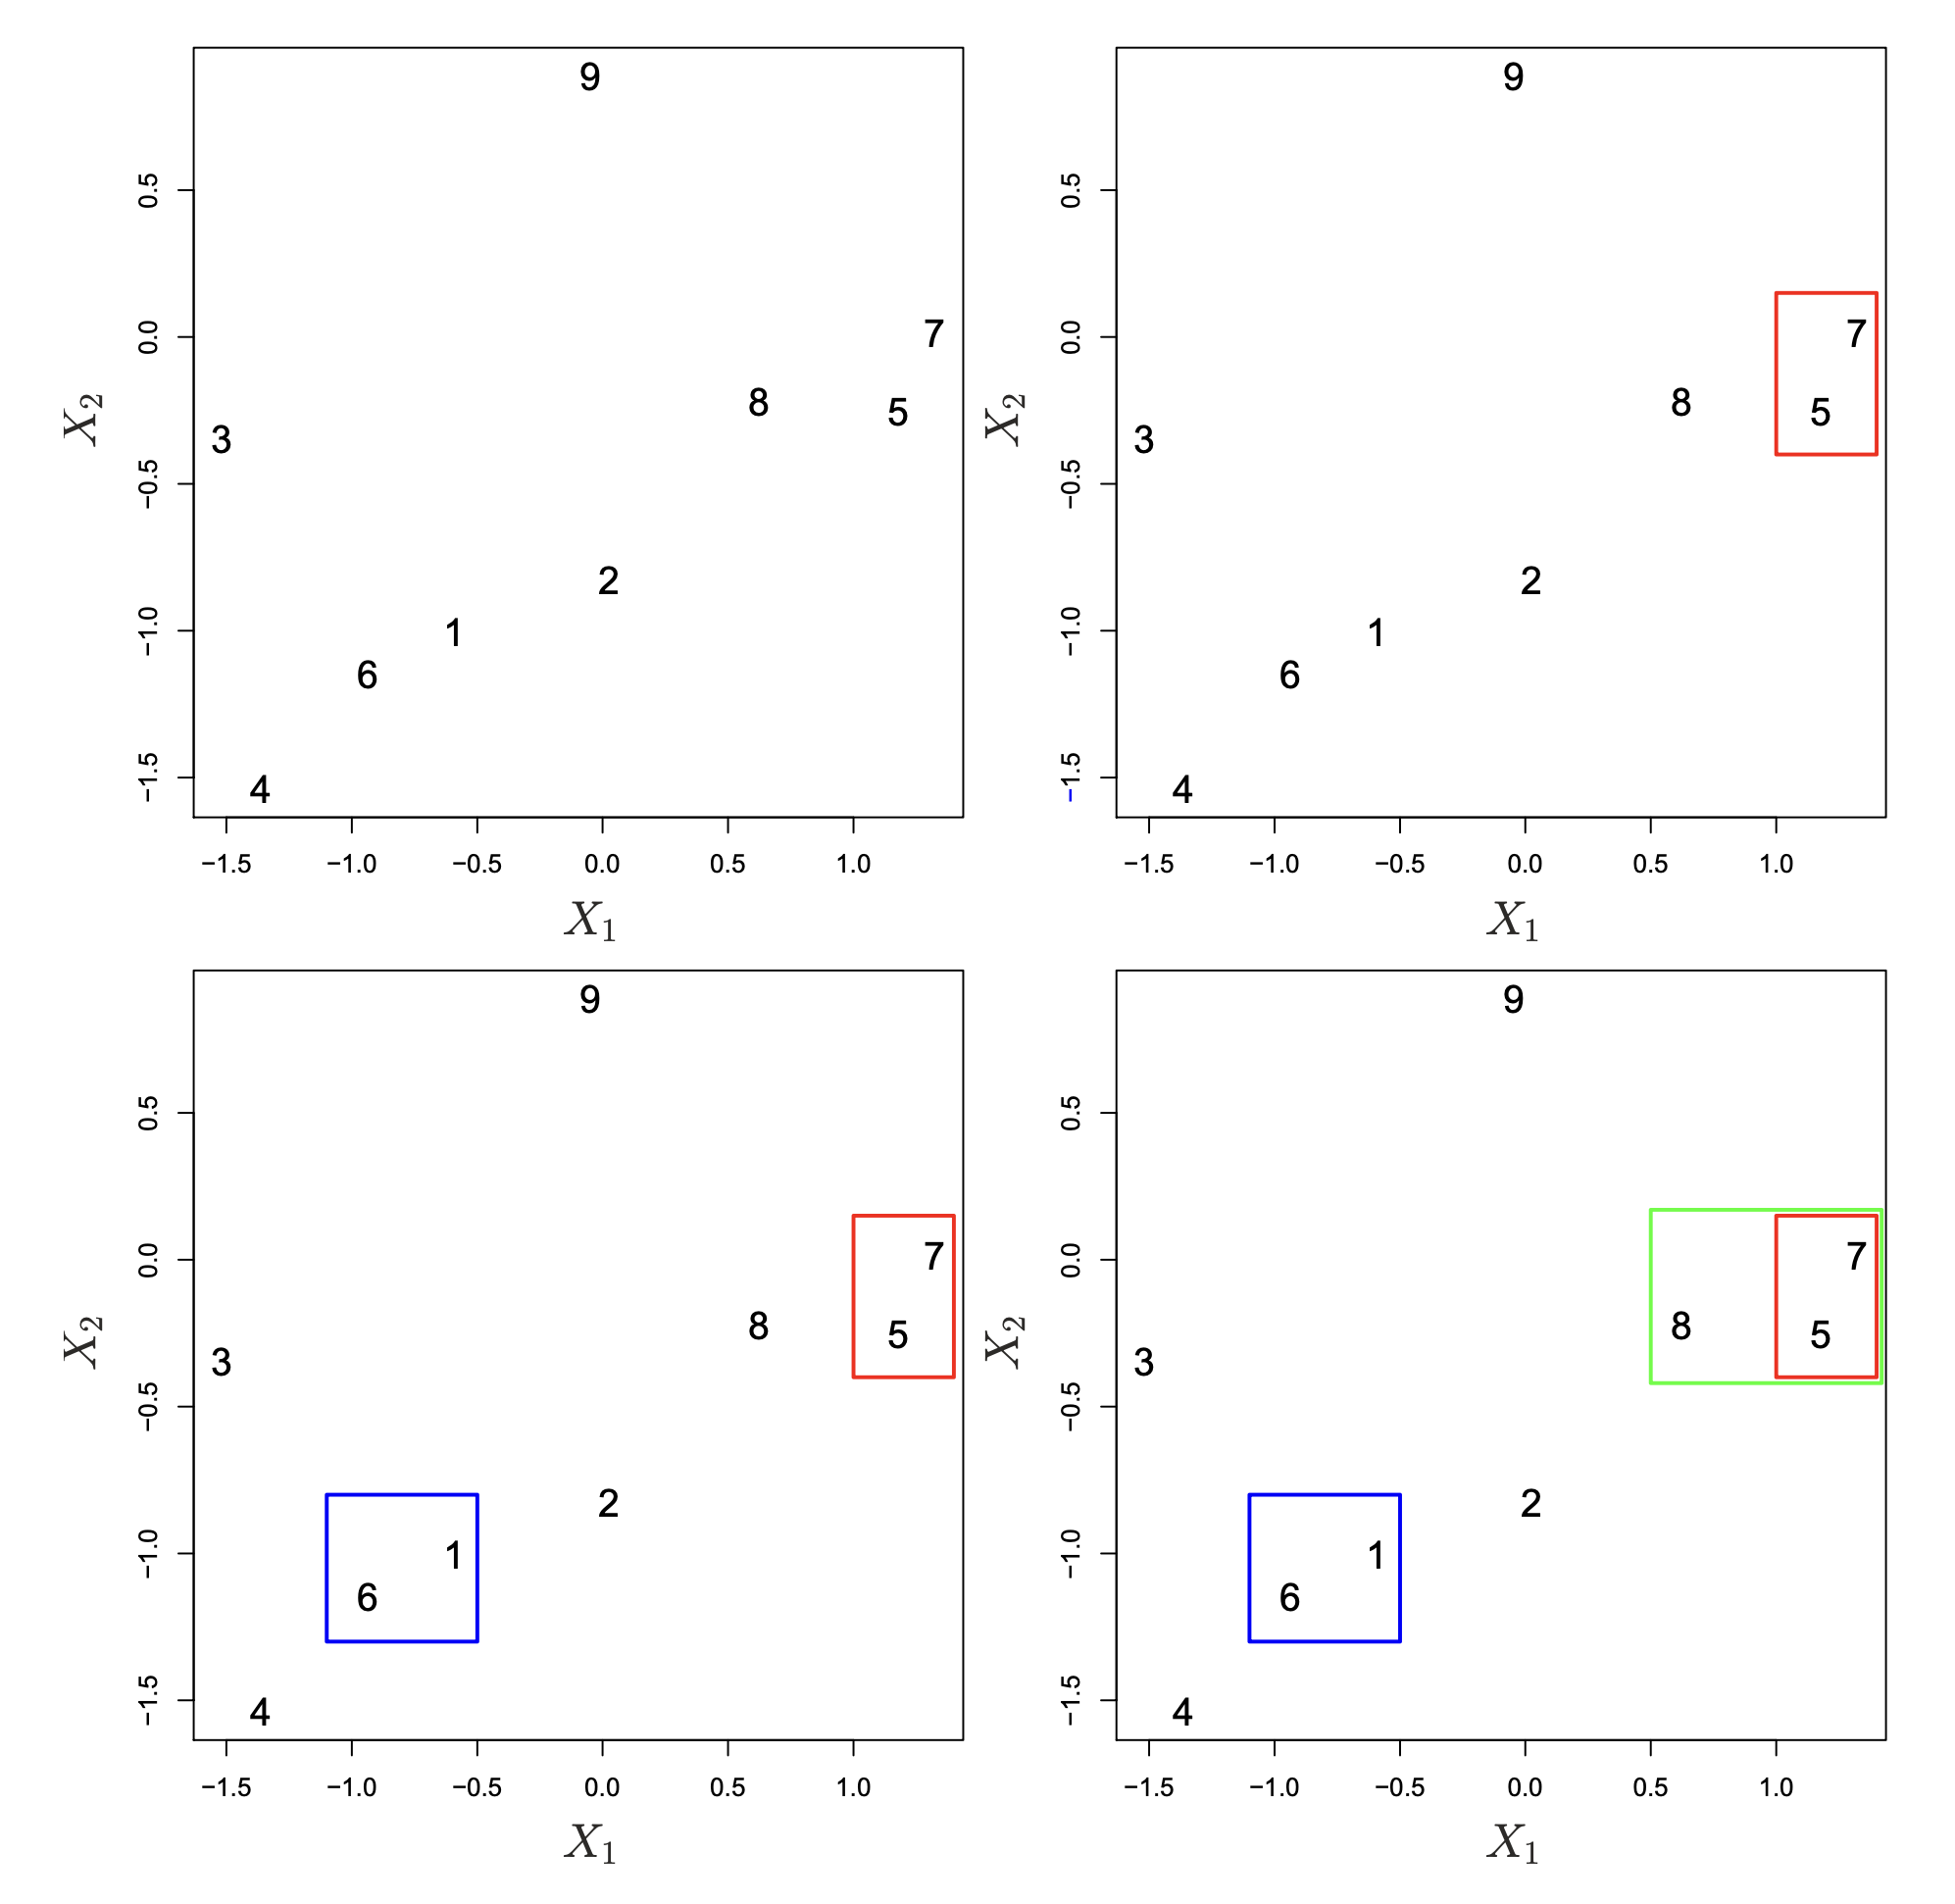
\includegraphics[width=0.7\textwidth]{assets/fig36.png}
    \caption{Hierarchical Clustering in R}
\end{figure}

\begin{figure}[H]
    \centering
    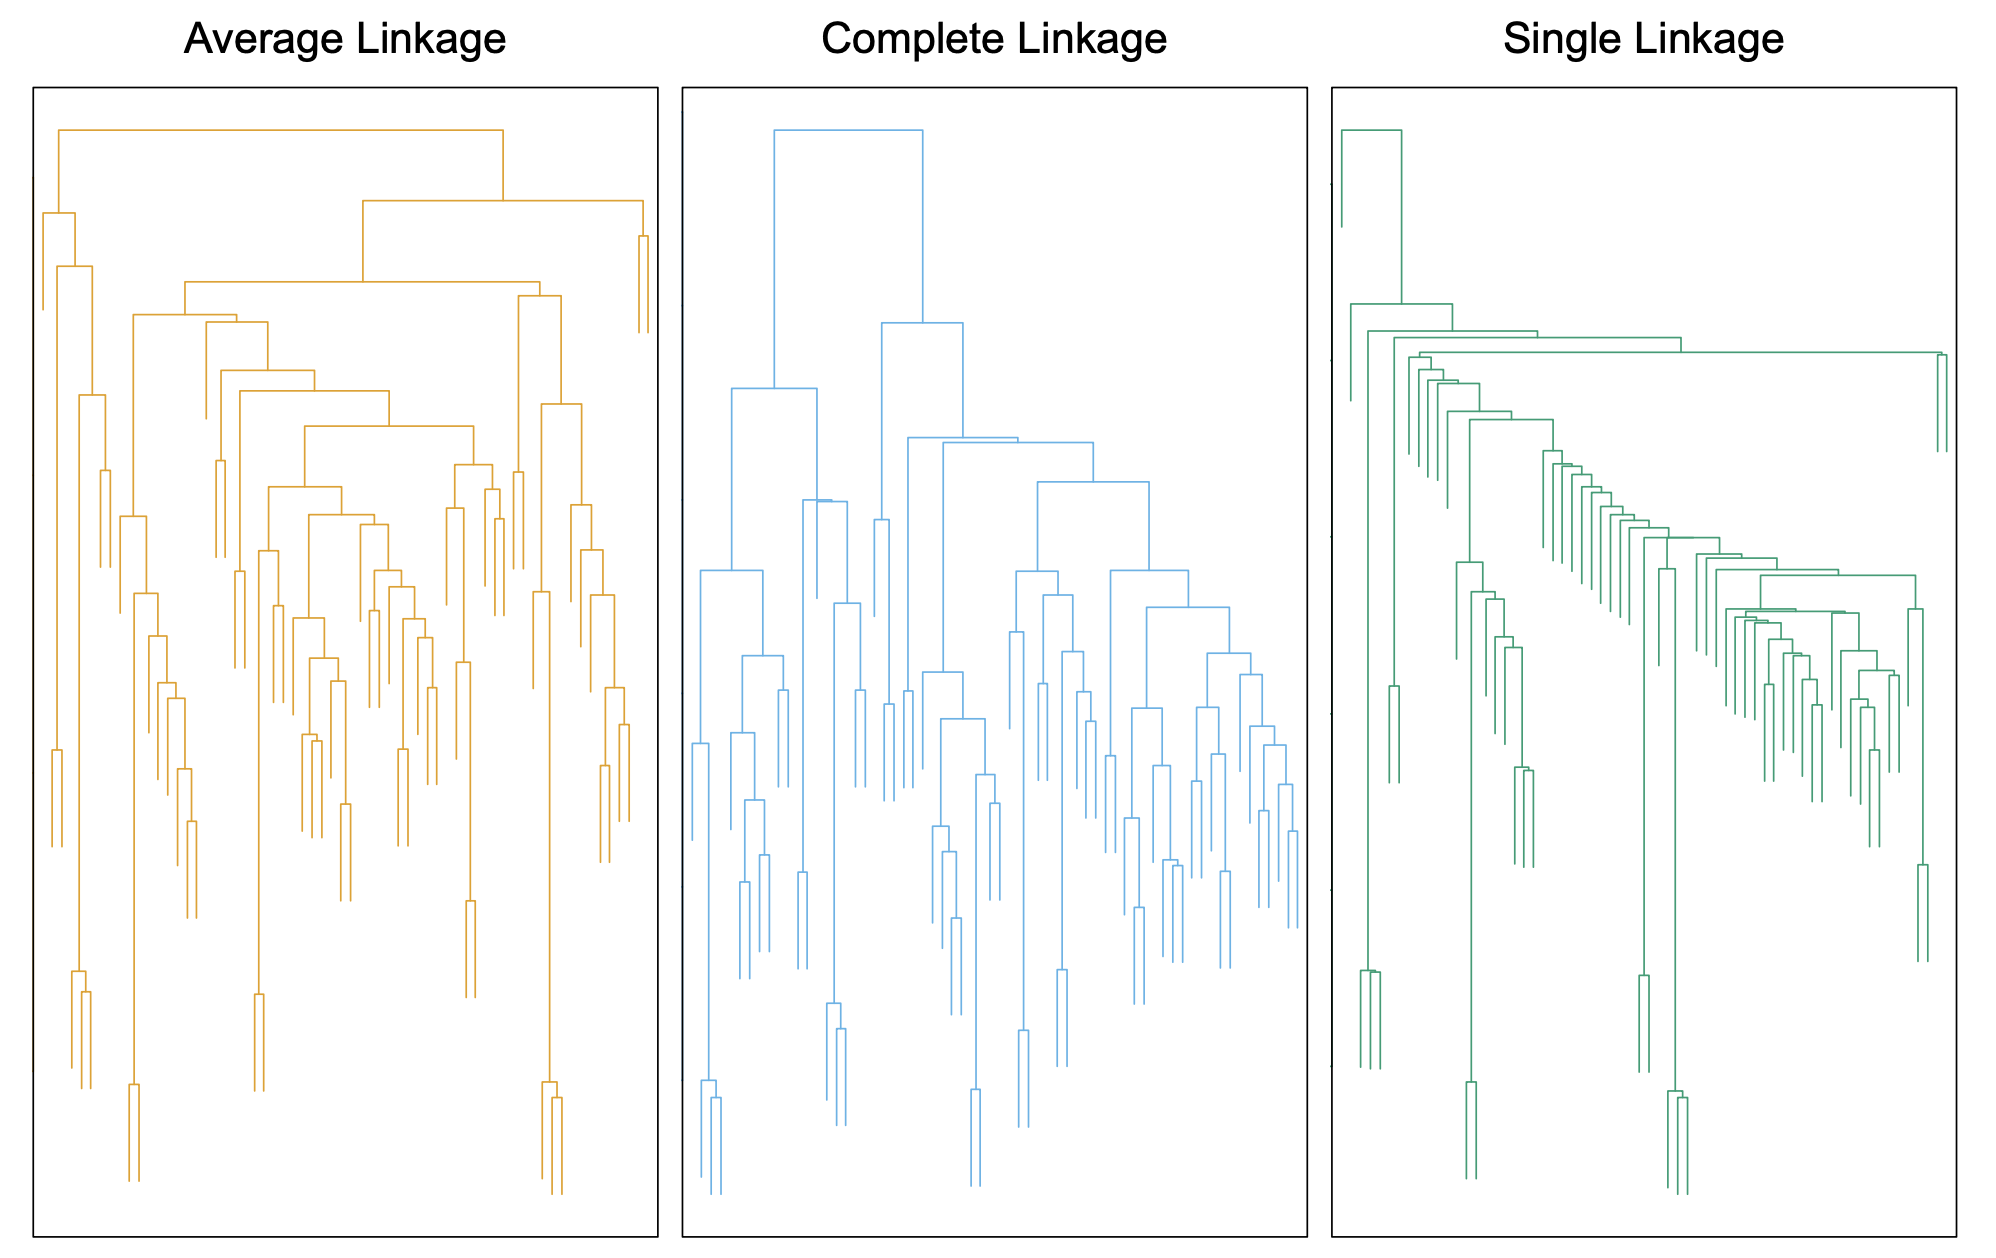
\includegraphics[width=0.8\textwidth]{assets/fig37.png}
    \caption{Distances in Hierarchical Clustering}
\end{figure}

\vspace{-1.5em}

\subsection{k-means}

\begin{definitionblock}[k-means]
K-means clustering is a simple and elegant approach for partitioning a data set into K distinct, non-overlapping clusters. To perform K-means clustering, we must first specify the desired number of clusters K; then the K-means algorithm will assign each observation to exactly one of the K clusters.
It is an iterative method in which:
\begin{itemize}
    \item you set k
    \item you set the initial centroids
    \item you assign each point to the closest centroid
    \item you update the centroids
    \item you repeat until convergence
\end{itemize}
A \textbf{centroid} is the average of all the points in a cluster.
\end{definitionblock}

This technique is not deterministic, due to the random initialization of the centroids. It is also sensitive to the initial centroids, so it is better to run it multiple times and choose the best result.

\begin{figure}[H]
    \centering
    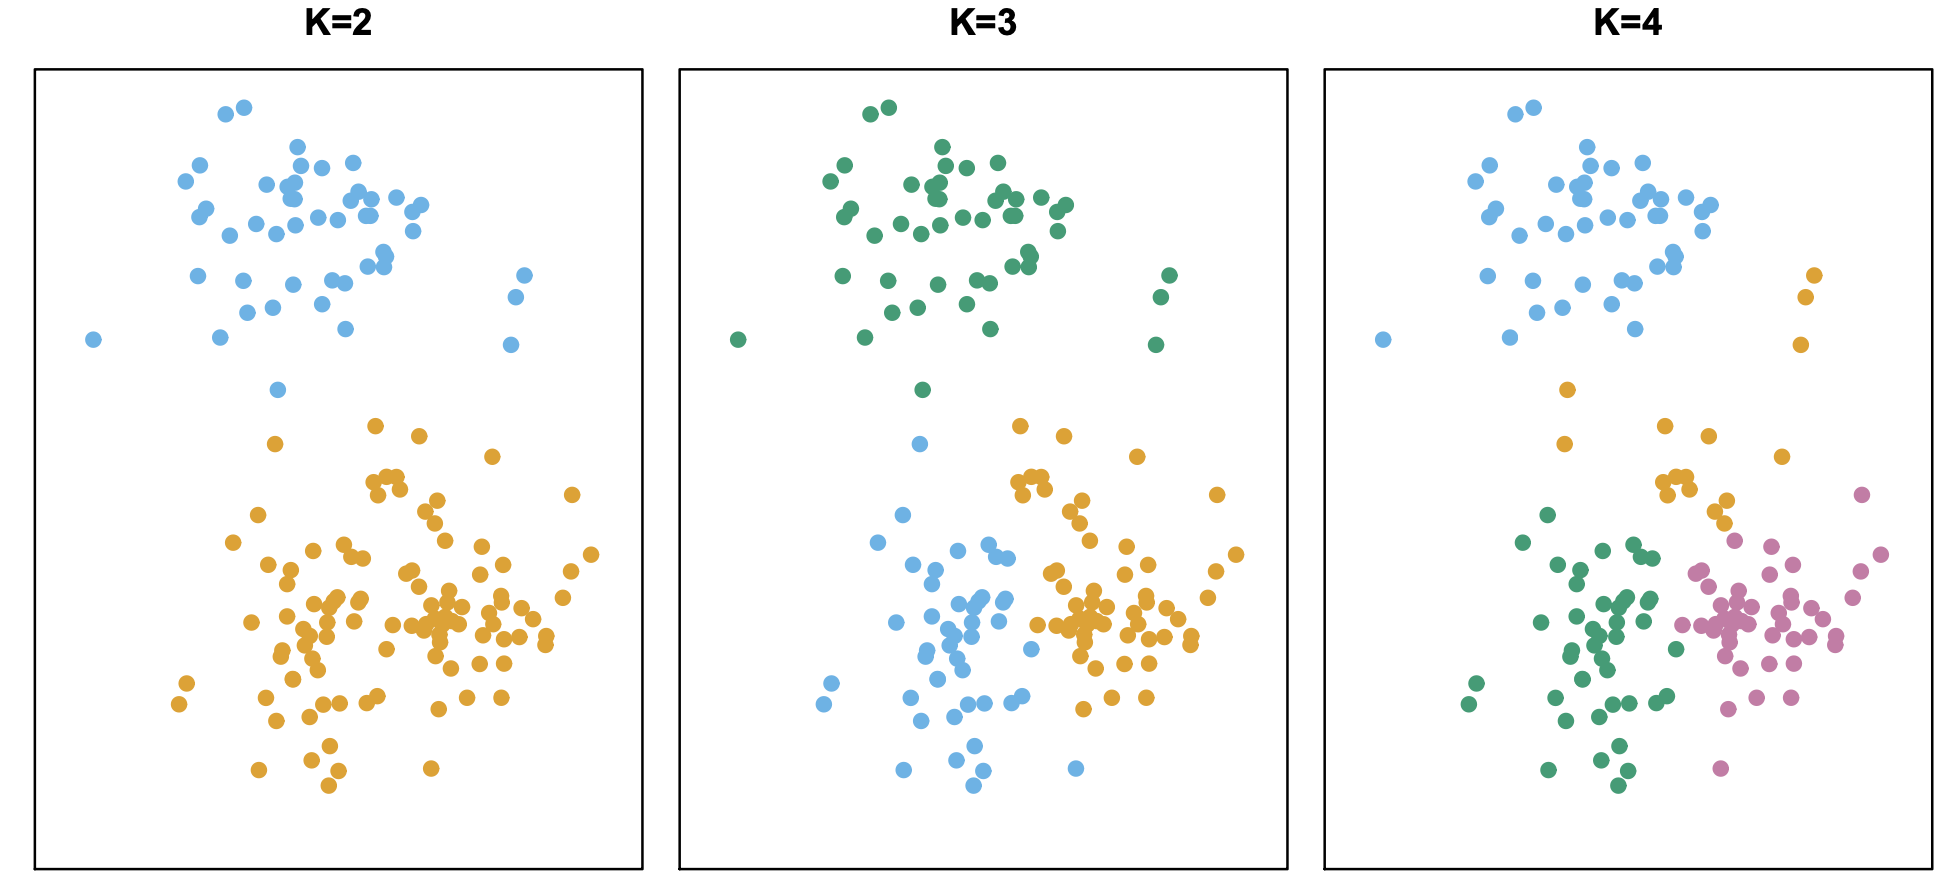
\includegraphics[width=0.8\textwidth]{assets/fig38.png}
    \caption{k-means}
\end{figure}
